\documentclass{article}
% \date{}
% 
\usepackage{listings}
\usepackage{listing}
 \usepackage{graphicx} 
 \usepackage[utf8]{inputenc}
 \oddsidemargin 0.0in 
 \textwidth 6.5in

 \begin{document}
% \maketitle

\begin{titlepage}

\begin{center}


% Upper part of the page

\includegraphics{images/logo.png}\\[1cm]

\textsc{\LARGE Faculdade de Ci\^{e}ncias e Tecnologia}\\[1.5cm]
\textsc{\LARGE Universidade Nova de Lisboa}\\[1.5cm]

\textsc{\Large Technical Report}\\[0.5cm]


% Title
\HRule \\[0.4cm]
{ \huge \bfseries DSLTrans Analytics}\\[0.4cm]

\HRule \\[1.5cm]

% Author and supervisor
\begin{minipage}{0.4\textwidth}
\begin{flushleft} \large
\emph{Authors:}\\
Bruno \textsc{Barroca}
\end{flushleft}
\end{minipage}
\vfill

% Bottom of the page
{\large \today}

\end{center}

\end{titlepage}


\clearpage

\begin{document}

This document reports an implementation of the verification
technique of DSLTrans' transformations as presented in
\cite{lucio:bar:2010}.

\section{Transformation Analysis Example}

First we have two languages that we want to translate.

\begin{figure}[h]
	\centering
	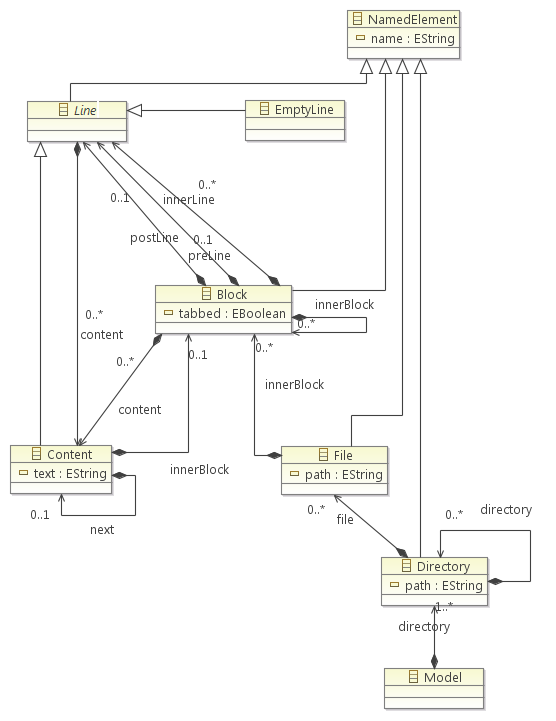
\includegraphics[scale=0.5]{images/text.png}
	\caption{Text MetaModel (in Ecore)}
	\label{fig:text}
\end{figure}


Our target language is called Text. This language has only
the concepts that are important to perform serializations to
a file system as shown in Figure\ref{fig:text}. Those are:
\begin{itemize}
	\item \textbf{Directory}: This represents the directories
	that are created when Text instances are executed.
	\item \textbf{File}: This represents the files that are
	created when Text instances are executed. These have to be
	included in some \textbf{Directory}.
	\item \textbf{Block}: This is a way to give an
	hierarchical structure to content in a \textbf{File}. When
	Text instances are executed, \textbf{Block}s are linearized
	to the containing \textbf{File}. This concept includes the
	idea of Tab so that users can perform indentation.
	\item \textbf{Content}: This is the concept that captures
	the actual text to be output when Text instances are
	executed. The \textbf{next} relationship indicates that
	there can be a sequence of \textbf{Content}s within the
	same line.
	\item \textbf{Block.preline,postLine and innerLine}: Each
	of these \textbf{Line}s will have at the end, a line feed
	or carriage return, again when Text instances are
	executed.
\end{itemize}

The Text is actually the only language we have that has its
own semantics implemented by means of a processor written in
Java. Moreover, this language is the base language of all of
our transformations --- which means that all of our
transformations have the ultimate specific objective to
produce textual code.

\begin{figure}[h!]
	\centering
	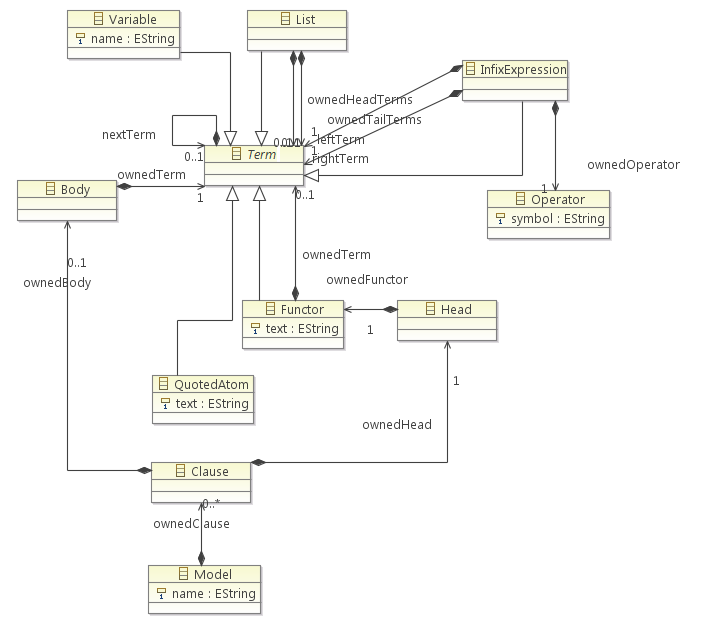
\includegraphics[scale=0.5]{images/mprolog.png}
	\caption{MProlog MetaModel (in Ecore)}
	\label{fig:mprolog}
\end{figure}

The source language of our transformation example is a
meta-modelled version of the Prolog language. We called it
MProlog, and its metamodel is shown in Figure
\ref{fig:mprolog}.

\subsection{The Transformation Specification}

Our transformation is specified in the DSLTrans language
(please refer to the DSLTrans' Manual for more details). We
stored our transformation in file
\textit{mprolog.ecore.dsltrans}. This specification is
structured into two layers. The first layer is called
\textit{Entities}, and the second one is called
\textit{Associations}.

One the one hand, the layer \textit{Entities} only handles
individual types (i.e no relations are matched) in all of its rules.
The rules are presented in Figures
\ref{fig:FactClauseRule},\ref{fig:ModelList},
\ref{fig:FunctorVariableRule}, and \ref{fig:lastrule}.

\begin{figure}[hb!]
\begin{minipage}[b]{0.5\linewidth}
\centering
		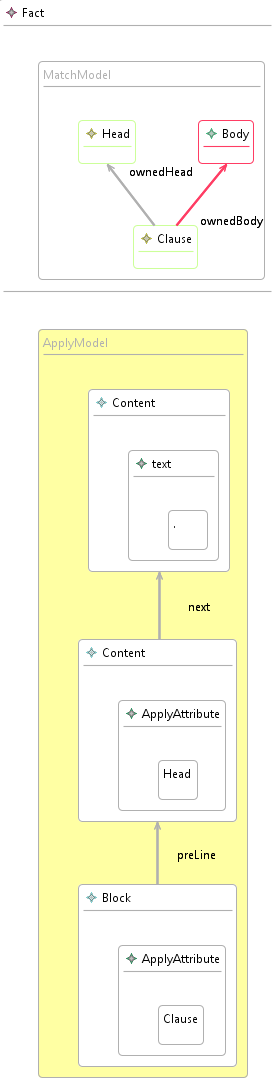
\includegraphics[scale=0.4]{images/FactRule.png}
\end{minipage}
\begin{minipage}[b]{0.5\linewidth}
		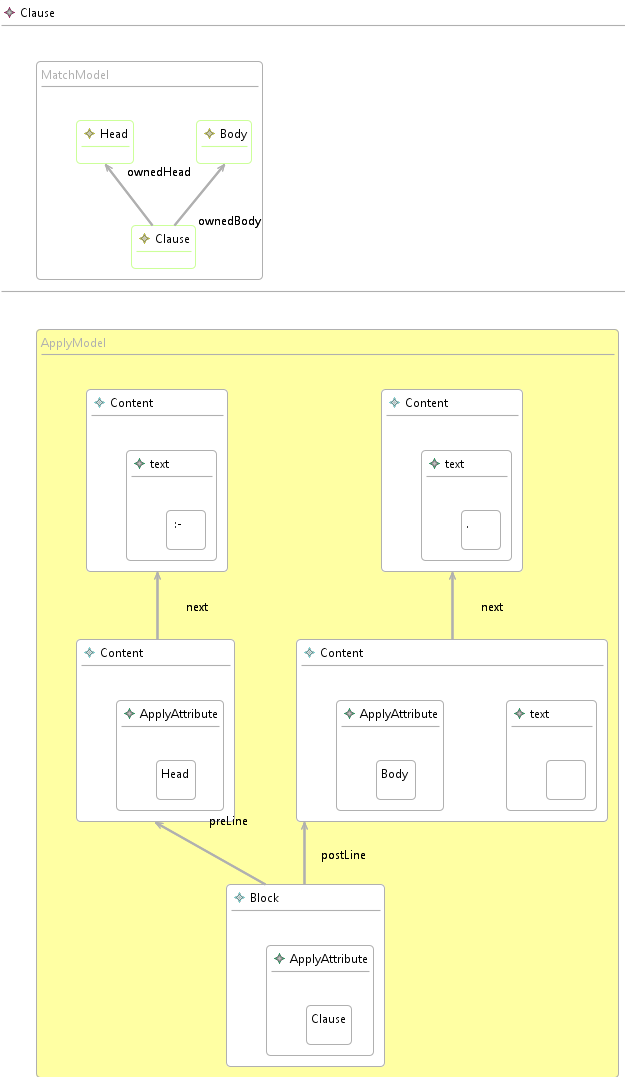
\includegraphics[scale=0.4]{images/ClauseRule.png}
\end{minipage}
\hspace{0.5cm}
	\caption{Fact Rule (on the left) and Clause Rule (on the
	right) expressed in DSLTrans. The \textit{Fact} Rule
	indicates that, when we have a \textbf{Clause} with a
	\textit{Head} but with no \textit{Body}, then we should
	create placeholders for the \textbf{Clause} (with the
	\textbf{Block}) and for its \textbf{Head} (with the
	\textbf{Content}), while closing the line with a dot $'.'$
	(again with a \textbf{Content}). The \textit{Clause} Rule
	indicates that, when we otherwise have a \textit{Body}
	within the \textit{Clause}, then we have to generate an
	additional symbol (by means of a \textbf{Content}: $':-'$
	to separate the \textit{Head} from the \textit{Body}. }
	\label{fig:FactClauseRule}
\end{figure}

\begin{figure}[hb!]
\begin{minipage}[b]{0.5\linewidth}
\centering
		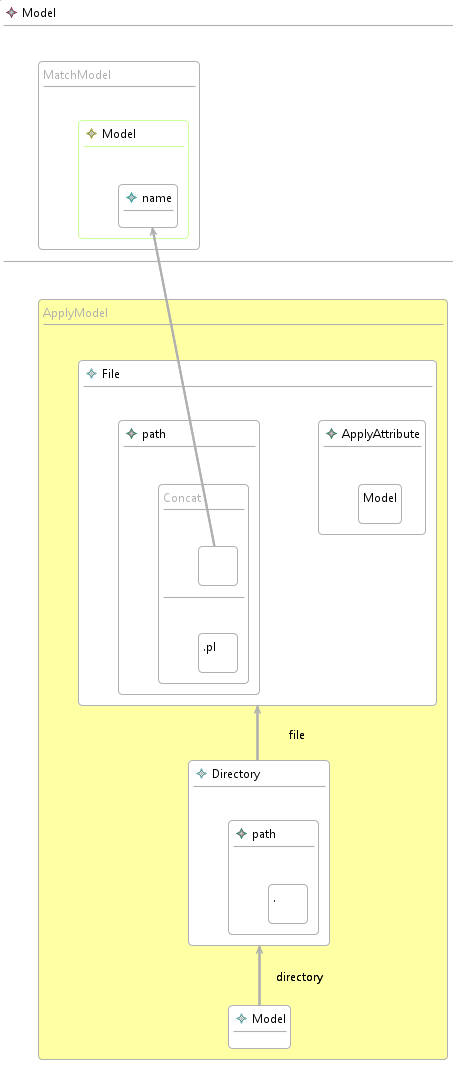
\includegraphics[scale=0.4]{images/ModelRule.png}
\end{minipage}
\begin{minipage}[b]{0.5\linewidth}
		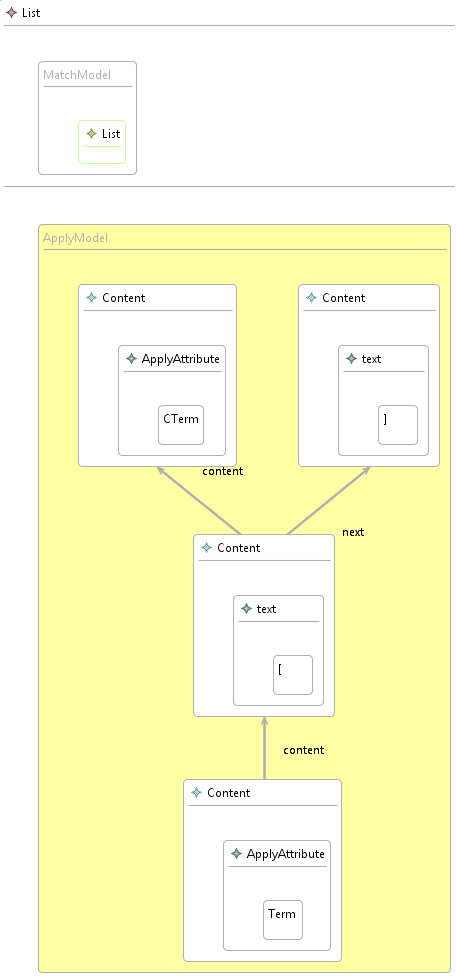
\includegraphics[scale=0.4]{images/ListRule.png}
\end{minipage}
\hspace{0.5cm}
	\caption{Model Rule (on the left) and List Rule (on the
	right) expressed in DSLTrans. The \textit{Model} Rule
	(on the left) indicates that the name of the
	\textit{Model} will be used as the name of the output .pl
	file. The \textit{List} Rule (on the right) indicates that
	whenever we find a \textbf{List}, then we must generate
	additional symbols to represent the the opening the List
	($'['$) and to close it ($']'$).}
	\label{fig:ModelList}
\end{figure}

\begin{figure}[h]
	\centering
	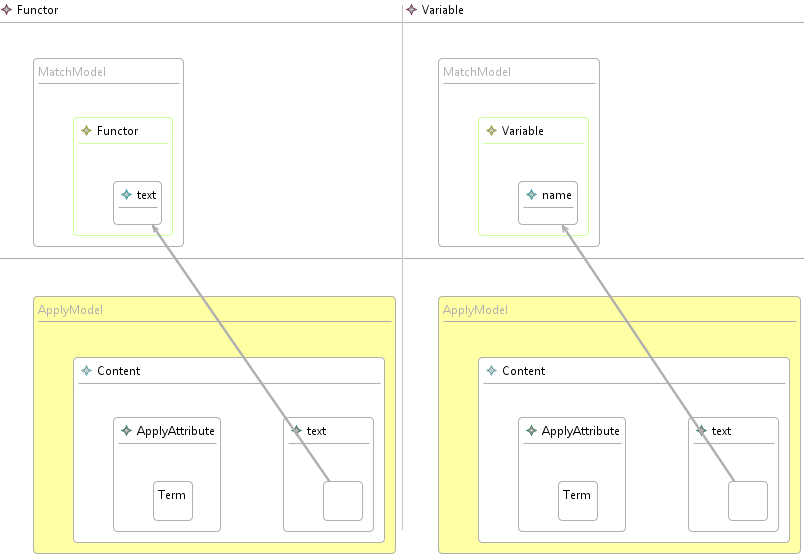
\includegraphics[scale=0.5]{images/FunctorVariableRule.png}
	\caption{DSLTrans' Rules for translating Functors and 
	Variables. Despite the fact that they have distinct
	types, when translated to Text, their values (text, and
	name) are just copied to the respective \textbf{Content}
	structures. However we can impose additional constraints
	stating for instance that all valid mprolog models should
	have variables with capital letters.}
	\label{fig:FunctorVariableRule}
\end{figure}

\begin{figure}[hb!]
	\centering
	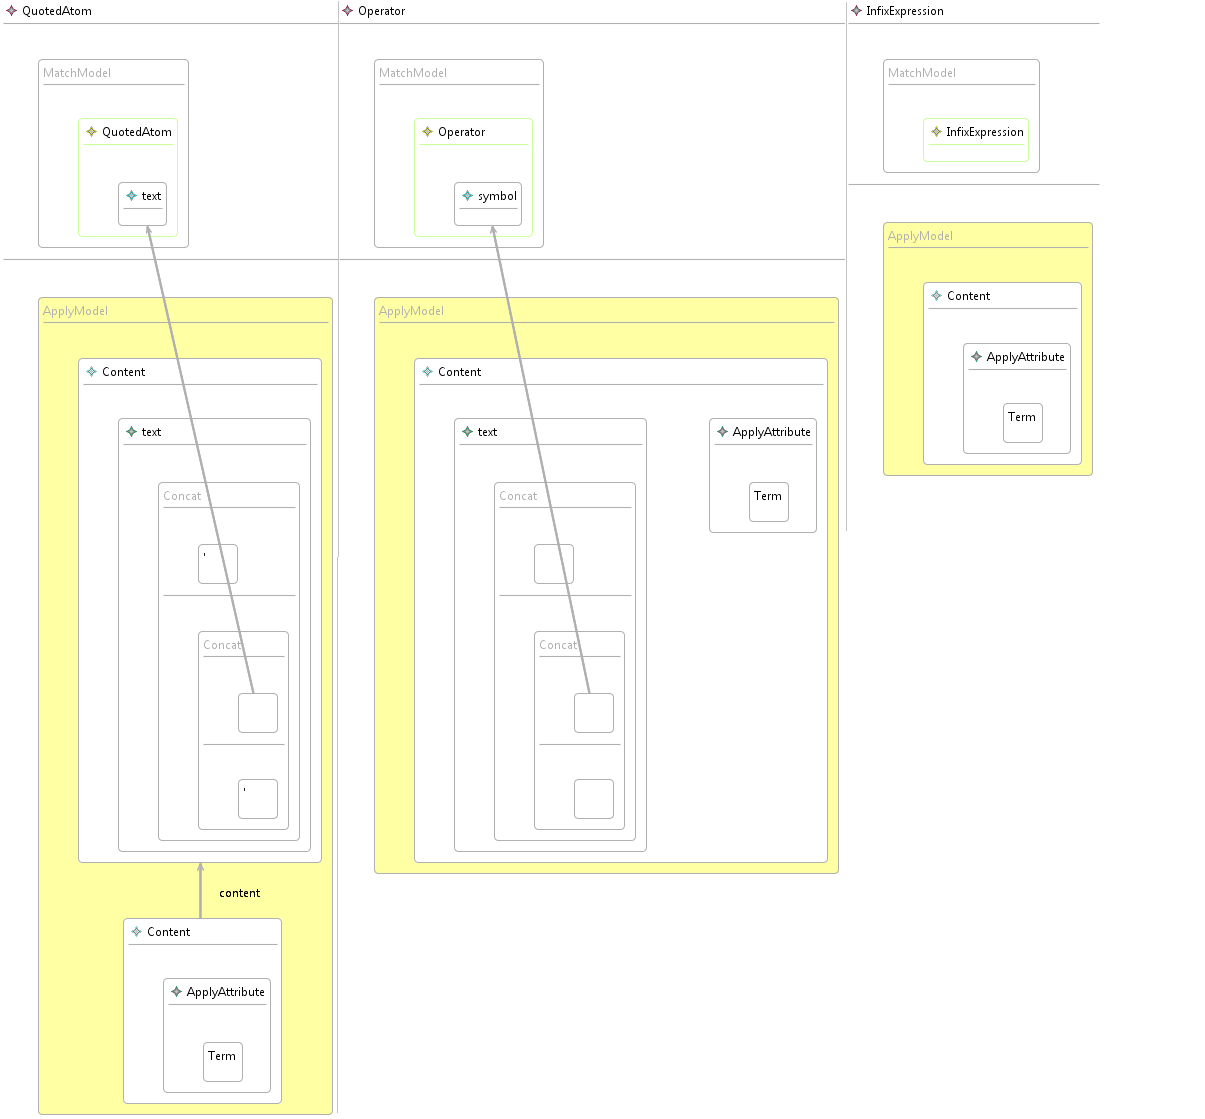
\includegraphics[scale=0.4]{images/LastRules.png}
	\caption{DSLTrans' Rules for translating QuotedAtoms,
	Operators and InfixExpressions. For each QuotedAtom, the
	translation generates quotes to surround the text. Also
	for each \textbf{Operator}, the symbol is copied to the
	\textbf{Content}, and finally, for the
	\textbf{InfixExpression}, only a placeholder is
	generated in order to encapsulate the whole structure as
	one single \textbf{Content}.}
	\label{fig:lastrule}
\end{figure}

In this approach we automatically generated from our
transformation specification mprolog.ecore.dsltrans a
Prolog file named mprolog.ecore.dsltrans.pl having only two
facts (one for each layer). The following is the encoding of the
$Entities$ layer expressed in Prolog.
\begin{lstlisting}
layer('Entities', id0, [
	rule('Fact', id8, 
		match_apply(
			graph([
				mc('mprolog','Clause', id11), 
				mc('mprolog', 'Head', id10)
			], 
			[
				mda('ownedHead', id11, id10)
			]), 
			graph([
				ac('Text','Block', id20), 
				ac('Text', 'Content', id19), 
				ac('Text', 'Content', id18)
			], [
				aa('preLine', id20, id19), 
				aa('next', id19, id18)
			]))),
	rule('List', id7, 
		match_apply(
			graph([
				mc('mprolog', 'List', id9)], []),
			graph([
				ac('Text', 'Content', id17), 
				ac('Text', 'Content', id16), 
				ac('Text', 'Content', id15), 
				ac('Text', 'Content', id14)
			], [
				aa('content', id17, id16), 
				aa('content', id16, id15),
				aa('next', id16, id14)
			]))), 
	rule('QuotedAtom', id6, 
		match_apply(
			graph([
				mc('mprolog', 'QuotedAtom', id8)
			], []), 
			graph([
				ac('Text', 'Content', id13), 
				ac('Text', 'Content', id12)], [
				aa('content', id13, id12)
			]))), 
	rule('Model', id5, 
		match_apply(
			graph([
				mc('mprolog', 'Model', id7)
			], []),
			graph([
				ac('Text', 'Model', id11), 
				ac('Text', 'Directory', id10), 
				ac('Text', 'File', id9)
			], [
				aa('directory', id11, id10), 
				aa('file', id10, id9)
			]))), 
	rule('Clause', id4, 
		match_apply(
			graph([
				mc('mprolog', 'Clause', id6),
				mc('mprolog', 'Head', id5), 
				mc('mprolog', 'Body', id4)
			],
			[
				mda('ownedHead', id6, id5), 
				mda('ownedBody', id6, id4)
			]), 
			graph([
				ac('Text', 'Block',id8), 
				ac('Text', 'Content', id7), 
				ac('Text', 'Content', id6), 
				ac('Text', 'Content', id5), 
				ac('Text', 'Content', id4)], 
			[
				aa('preLine', id8, id7), 
				aa('next', id7, id6), 
				aa('postLine', id8, id5), 
				aa('next', id5, id4)
			]))), 
	rule('Functor', id3, 
		match_apply(
			graph([
				mc('mprolog', 'Functor', id3)
			], []),
			graph([
				ac('Text', 'Content', id3)
			], []))),
	rule('Variable', id2, 
		match_apply(
			graph([
				mc('mprolog', 'Variable', id2)
			], []),
			graph([
				ac('Text', 'Content', id2)
			], []))),
	rule('InfixExpression', id1, 
		match_apply(
			graph([
				mc('mprolog', 'InfixExpression', id1)
			],
			[]), 
			graph([
				ac('Text', 'Content', id1)
				], []))),
	rule('Operator', id0, 
		match_apply(
			graph([
				mc('mprolog','Operator', id0)
				], []), 
			graph([
				ac('Text','Content', id0)
			], [])))
		], id0).

\end{lstlisting}

These facts represents our transformation under analysis.
The layer facts are in the form $layer(name, id, ruleList,
idpar)$, where $name$ is the actual name of the layer, $id$
is a generated instance identifier for the layer, $ruleList$
is a list of rules, and $idpar$ is the identifier of the
previous layer. If the previous layer identifier is the same
as the its own identifier, then the layer has no previous
layer. In this case, the previous layer of
layer $Associations$ is layer $Entities$. Each rule is in
the form $rule(name, id,
match_apply(graph(V,E),graph(V',E'))$, where $name$ is the name of the rule, $id$ is its unique identifier, $V$ and $E$
are match vertices and match edges respectively, and $V'$
and $E'$ are apply vertices and apply edges respectively.
 Match vertices have a general shape of
 $mc(package,class,id)$, where $package$ and $class$ form
 the vertice type and $id$ represents its unique identifier.
 Match edges have a general shape of $e(name,ids,idt)$,
 where $name$ is the name of the edge, $ids$ and $idt$ are
 the ids of the source and target vertices, and $e \in \{
 br, mda, mia\}$ --- i.e represents the kinds of possible
 match edges backward restriction, positive match
 association and indirect match association.
To encode apply vertices we only use the $ac$ functor (i.e
apply class), and to encode apply edges, we only use the
$aa$ functor (i.e apply association).
Note that for simplicity reasons, we neglet negative
conditions from our encoding. 

One the other hand, the layer \textit{Associations} handles
with all the relations defined in the metamodel of our
source language (i.e the MProlog), in all of its rules.
These rules are presented in Figures
\ref{fig:leftrightnext}, \ref{fig:headtailclausefunctor},
and \ref{fig:term}.

\begin{figure}[hb!]
	\centering
	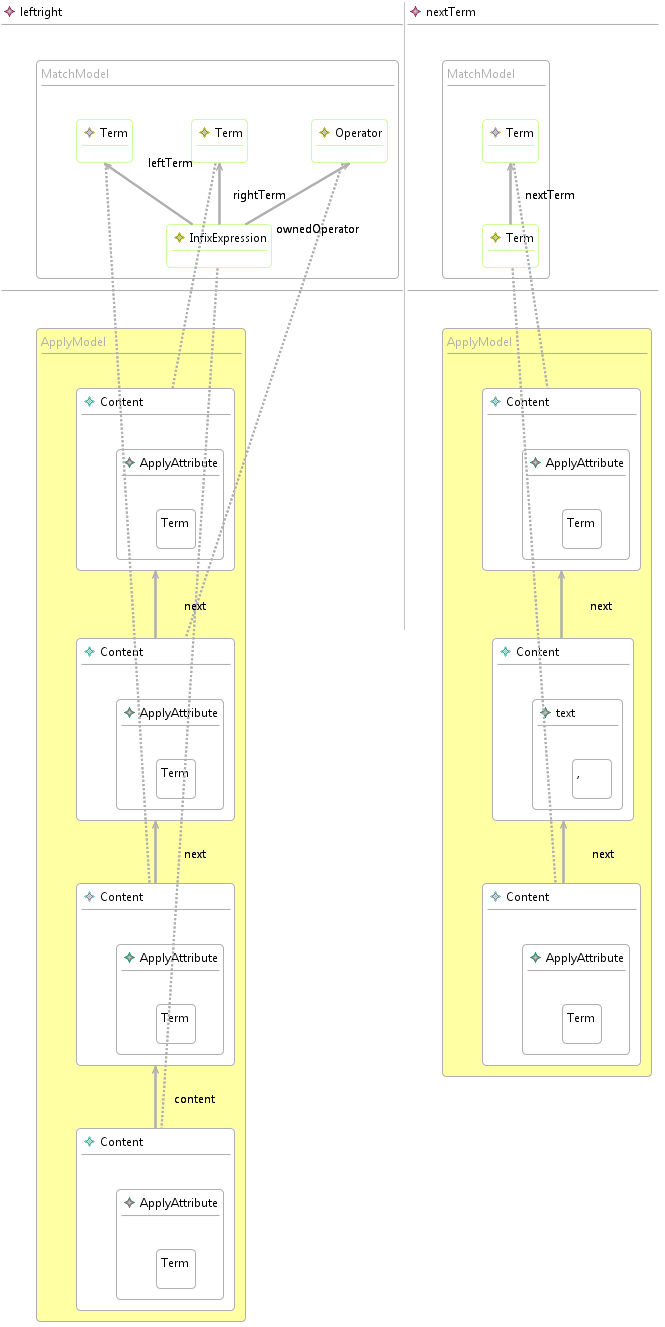
\includegraphics[scale=0.4]{images/leftrightnext.png}
	\caption{DSLTrans' Rules for translating the
	left and right relation of the \textbf{InfixExpression},
	and the nextTerm relation of generic \textbf{Terms}. In
	the first case, the generated \textbf{Contents} from the
	\textit{Entities} layer are organized so that the
	\textbf{Content} of the right term is preceded by the
	\textbf{Content} of the operator, and the
	\textbf{Content} of the operator is preceded by the
	\textbf{Content} of the left term. In what matters to the
	nextTerm relation, it is translated into an additional
	symbol (a $','$) to separate both terms in the sequence.}
	\label{fig:leftrightnext}
\end{figure}

\begin{figure}[hb!]
	\centering
	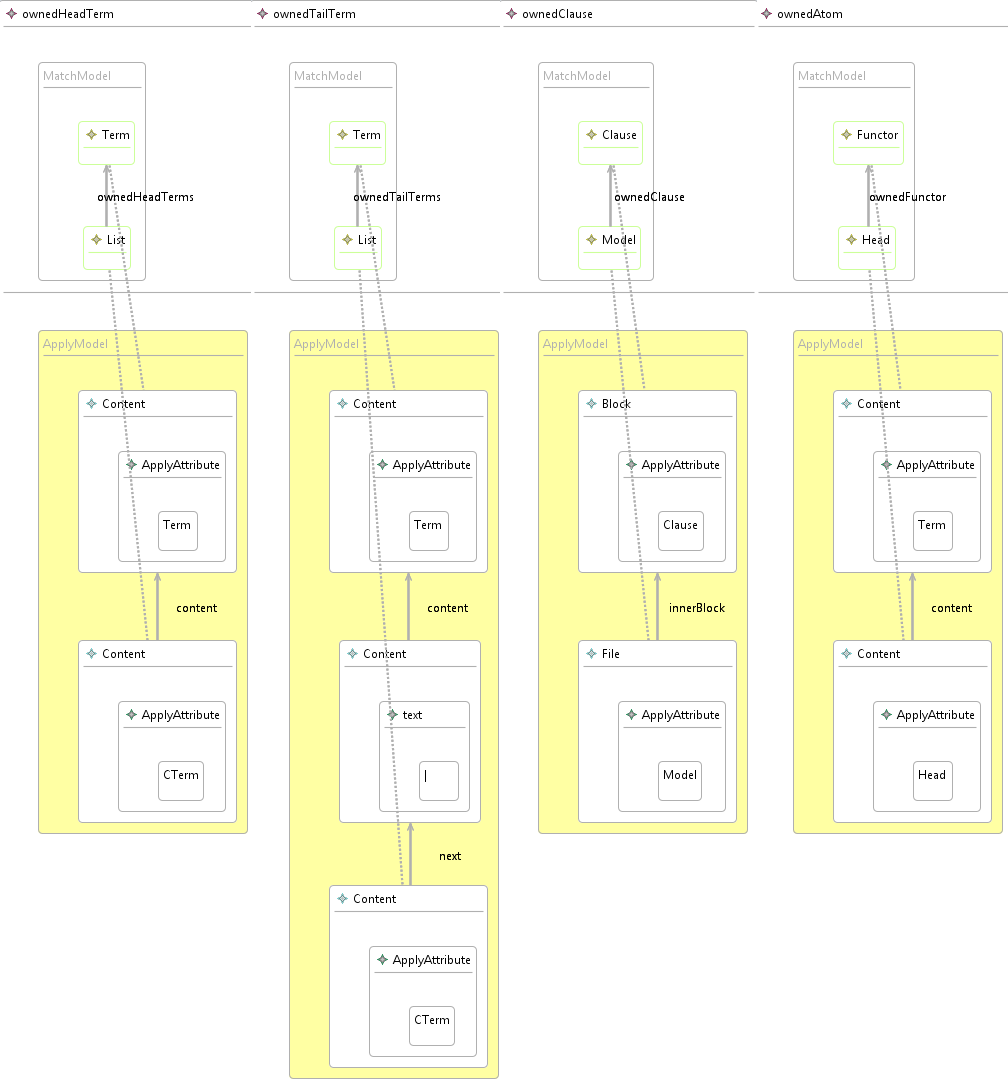
\includegraphics[scale=0.4]{images/headtailclausefunctor.png}
	\caption{DSLTrans' Rules for translating the
	head and tail relations of a \textbf{List} (on the left),
	clause relation of a \textbf{Model} (on the center) and
	functor relation of a \textbf{Clause} (on the right).
	Notice that on the case of the tail relation, we have to
	introduce an additional symbol ($'|'$) for the list
	separator.}
	\label{fig:headtailclausefunctor} 
\end{figure}

\begin{figure}[hb!]
	\centering
	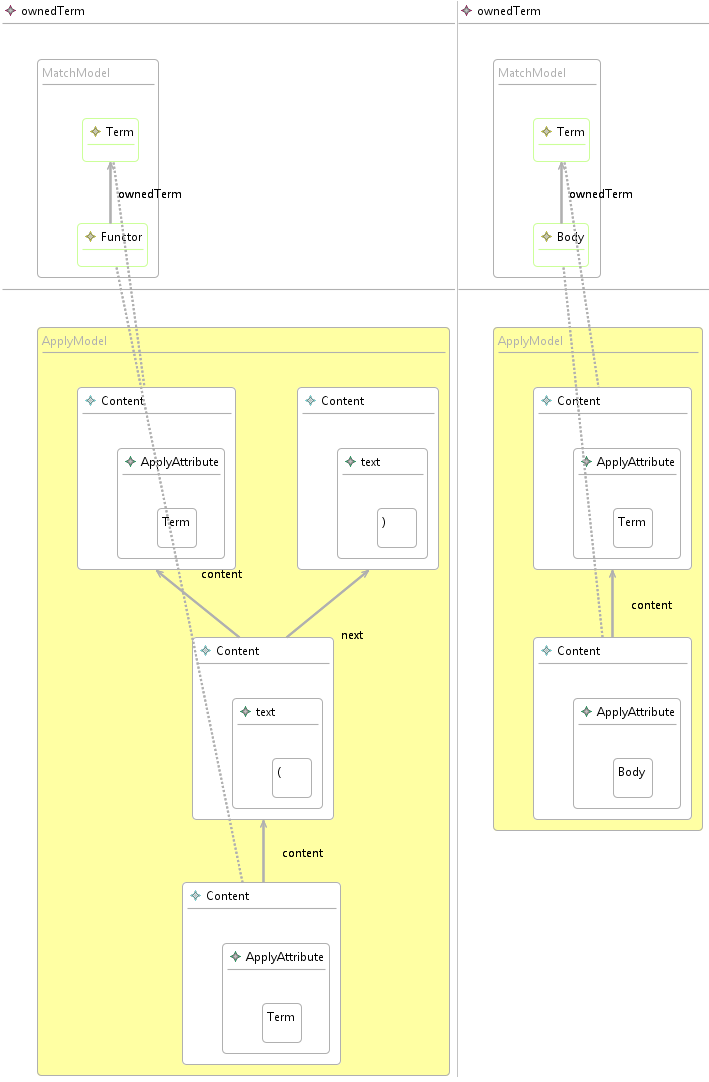
\includegraphics[scale=0.4]{images/term.png}
	\caption{DSLTrans' Rules for translating the
	ownedTerm relations of both a \textbf{Functor} (on the
	left), and a \textbf{Body} (on the right). In the case of
	the \textbf{Functor} the translation introduces the
	parenthesis symbols ($'('$ and $')'$).}
	\label{fig:term} 
\end{figure}

The following is the layer fact corresponding to the
encoding of the layer $Associations$ expressed in Prolog:

\begin{lstlisting}
layer('Associations', id1, [
	rule('ownedAtom', id16, 
		match_apply(
			graph([
				mc('mprolog','Head', id29), 
				mc('mprolog', 'Functor', id28)
			], [
				br('_', id29, id42), 
				br('_', id28, id41),
				mda('ownedFunctor', id29, id28)
			]), 
			graph([
				ac('Text','Content', id42), 
				ac('Text', 'Content', id41)
			], [
				aa('content', id42, id41)
			]))), 
	rule('nextTerm', id15,
		match_apply(
			graph([
				mc('mprolog', 'Term', id27),
				mc('mprolog', 'Term', id26)
			], [
				br('_', id27, id40),
				br('_', id26, id39), 
				mda('nextTerm', id27, id26)
			]),
			graph([
				ac('Text', 'Content', id40), 
				ac('Text', 'Content', id39), 
				ac('Text', 'Content', id38)
			], [
				aa('next', id40, id38), 
				aa('next', id38, id39)
			]))),
	rule('ownedHeadTerm', id14,
		match_apply(
			graph([
				mc('mprolog', 'List', id25),
				mc('mprolog', 'Term', id24)
			], [
				br('_', id25, id37), 
				br('_', id24, id36), 
				mda('ownedHeadTerms', id25, id24)
			]), 
			graph([
				ac('Text', 'Content', id37), 
				ac('Text', 'Content', id36)
			], [
				aa('content', id37, id36)
			]))), 
	rule('ownedTerm', id13, 
		match_apply(
			graph([
				mc('mprolog', 'Functor', id23),
				mc('mprolog', 'Term', id22)
			], [
				br('_', id23, id35),
				br('_', id22, id34), 
				mda('ownedTerm', id23, id22)
			]),
			graph([
				ac('Text', 'Content', id35), 
				ac('Text', 'Content', id34), 
				ac('Text', 'Content', id33), 
				ac('Text', 'Content', id32)
			], [
				aa('content', id35, id33), 
				aa('content', id33, id34),
				aa('next', id33, id32)
			]))), 
	rule('ownedTerm', id12, 
		match_apply(
			graph([
				mc('mprolog', 'Body', id21),
				mc('mprolog', 'Term', id20)
				], [
				br('_', id21, id31),
				br('_', id20, id30), 
				mda('ownedTerm', id21, id20)
			]), 
			graph([
				ac('Text', 'Content', id31),
	 			ac('Text', 'Content', id30)
	 		], [
	 			aa('content', id31, id30)
	 		]))), 
	 rule('ownedClause', id11, 
	 	match_apply(
	 		graph([
				 mc('mprolog', 'Model', id19), 
				 mc('mprolog', 'Clause', id18)
			 ], [
				 br('_', id19, id29), 
				 br('_', id18, id28), 
				 mda('ownedClause', id19, id18)
			 ]), 
	 		graph([
				 ac('Text', 'File', id29), 
				 ac('Text', 'Block', id28)
			 ], [
				 aa('innerBlock', id29, id28)
			 ]))), 
	 rule('ownedTailTerm', id10, 
	 	match_apply(
	 		graph([
				 mc('mprolog', 'List', id17), 
				 mc('mprolog', 'Term', id16)
			 ], [
				 br('_', id17, id27), 
				 br('_', id16, id26), 
				 mda('ownedTailTerms', id17, id16)
			 ]), 
			 graph([
				 ac('Text', 'Content', id27), 
				 ac('Text', 'Content', id26), 
				 ac('Text', 'Content', id25)
			 ], [
				 aa('next', id27, id25), 
				 aa('content', id25, id26)
			 ]))), 
	 rule('leftright', id9, 
		 match_apply(
	 		graph([
				 mc('mprolog', 'InfixExpression', id15), 
				 mc('mprolog', 'Term', id14), 
				 mc('mprolog', 'Term', id13), 
				 mc('mprolog', 'Operator', id12)
			 ], [
				 br('_', id15, id24), 
				 br('_', id14, id22), 
				 br('_', id12, id21), 
				 br('_', id13, id23), 
				 mda('leftTerm', id15, id14), 
				 mda('rightTerm', id15, id13), 
				 mda('ownedOperator', id15, id12)
			 ]), 
			 graph([
				 ac('Text', 'Content', id24), 
				 ac('Text', 'Content', id23), 
				 ac('Text', 'Content', id22), 
				 ac('Text', 'Content', id21)
			 ], [
				 aa('content', id24, id22), 
				 aa('next', id22, id21), 
				 aa('next', id21, id23)
	 ])))], id0).
\end{lstlisting}


\subsection{The Transformation Property}

In this particular example, we have used the same
DSLTrans' syntax to express a property that we want to check
in order to validate our transformation. In Figure
\ref{fig:property} we show a property that a language
engineer should have in his/her mind to validate the
above presented transformation. In this case, the language
engineer expects (with the above presented
transformation) that any \textbf{Clause} with at least one
head with a \textbf{Functor}, and a \textbf{Body}, will
generate a particular kind of structure of \textbf{Block}
with \textbf{Contents} inside, having also both the $'.'$
and $':-'$ symbols.

\begin{figure}[hb!]
	\centering
	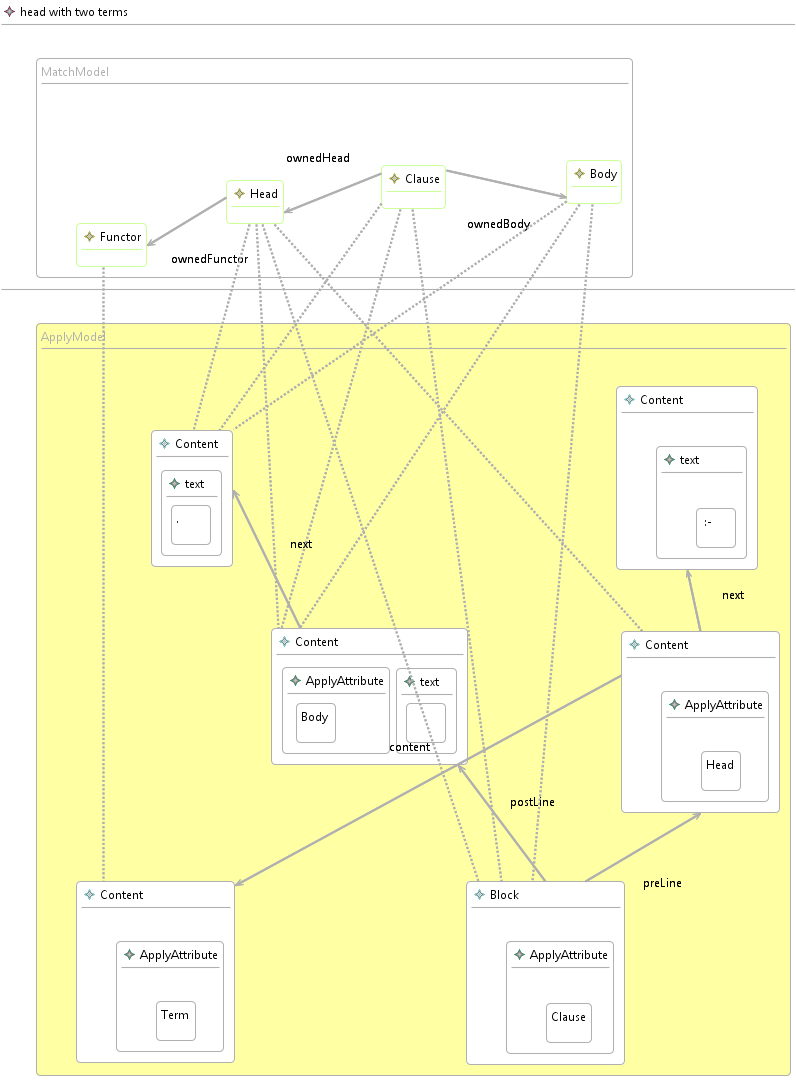
\includegraphics[scale=0.4]{images/myproperty.png}
	\caption{A DSLTrans' property.}
	\label{fig:property} 
\end{figure}

Similarly, we encoded our property into Prolog. To
distinguish between our transformation under analysis'
layers from the property, we used another fact called
'property' having the general form of $property(RuleList)$,
where $RuleList$ is a list of rules with the same shape as
presented above. The following is the respective Prolog
encoding of the above presented property:

\begin{lstlisting}
property([
	rule('head with two terms', id0,
			match_apply(
				graph([
					mc('mprolog', 'Functor', id3),
					mc('mprolog', 'Head', id2), 
					mc('mprolog', 'Clause', id1), 
					mc('mprolog', 'Body', id0)
				], [
					br('_', id3, id5),
					br('_', id2, id4), 
					br('_', id0, id3), 
					br('_', id1, id3), 
					br('_', id2, id3), 
					br('_', id0, id2), 
					br('_', id1, id2), 
					br('_', id2, id2), 
					br('_', id2, id0), 
					br('_', id1, id0), 
					br('_', id0, id0), 
					mda('ownedHead', id1, id2), 
					mda('ownedBody', id1, id0), 
					mda('ownedFunctor', id2, id3)
				]), 
				graph([
					ac('Text', 'Content', id5), 
					ac('Text', 'Content', id4), 
					ac('Text', 'Content', id3), 
					ac('Text', 'Block', id2), 
					ac('Text', 'Content', id1), 
					ac('Text', 'Content', id0)
				], [
					aa('preLine', id2, id4), 
					aa('next', id4, id1), 
					aa('postLine', id2, id3), 
					aa('content', id4, id5), 
					aa('next', id3, id0)
	])))]).
\end{lstlisting}

\section{Performing the Analysis}

In a translation analysis, each
symbolic state represents \textit{(i)} a combination of
the translation's rule-applications, and \textit{(ii)} a
combination of merges between two or more match (or apply)
nodes that reference the same source (or target) language's
type, on two or more of the applied translation's rules.
Therefore, each translation's symbolic state is formed by a
pair of patterns from both source and target language.
In Figure \ref{fig:dsltransstate}, it is shown one of
symbolic states resulting from the translation analysis
performed on the presented transformation.

\begin{figure}[hb!]
	\centering
	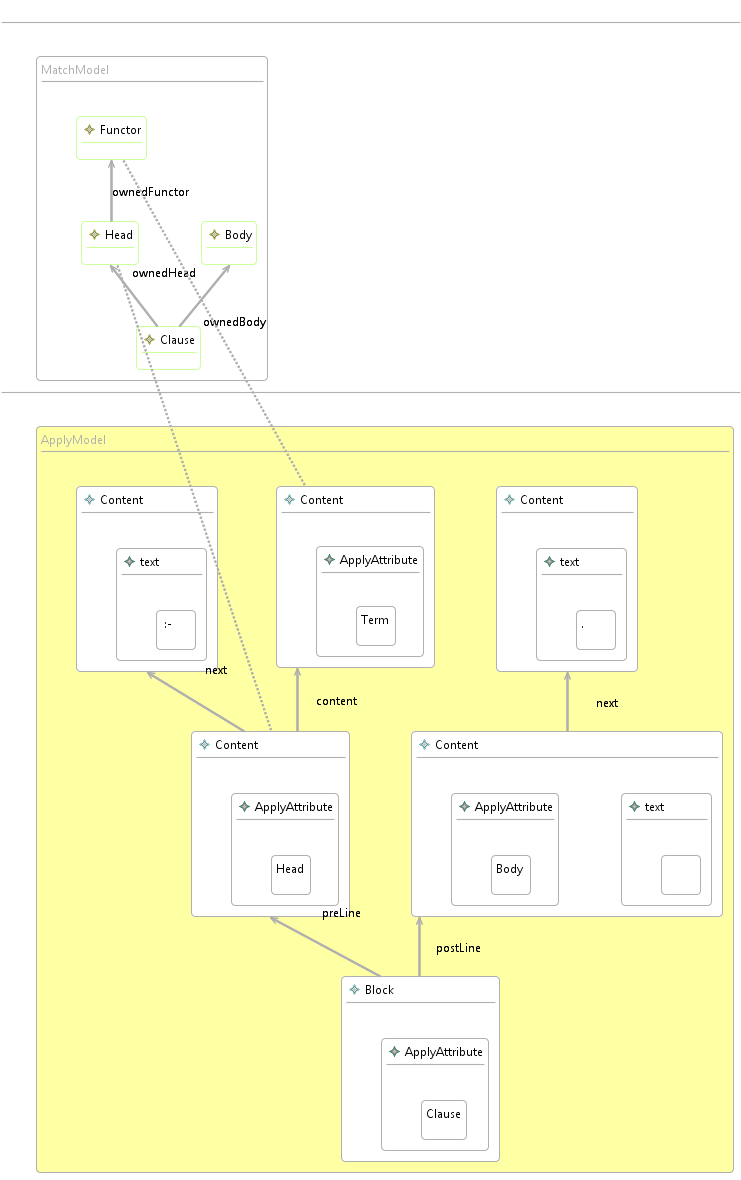
\includegraphics[scale=0.4]{images/mprolog_state.png}
	\caption{A symbolic state resulting from the merge
	of two DSLTrans' Rules: 'Clause' and 'ownedAtom'.}
	\label{fig:dsltransstate} 
\end{figure}

Notice that in this symbolic state, both the match elements
'Head' and 'Functor' on both rules were merged together with
their respective apply elements. This state represents the
case where both the rules were applied and these elements
were the same in the input model. Therefore, in this
particular case the resulting apply model is shown in the
Apply Model section.

\subsection{On-the-fly technique}
Instead of generating all the state-space of the
transformation, our first approach is to generate a
small symbolic state-space according to the property that we
want to prove.

\begin{lstlisting}
build_evidence(
	evidence(
		LayerName,IDL,
		RuleName,IDR,
		PropertyName,IDP,
		GT
	)
):- 
	property(LP),
	layer(LayerName,IDL,LR,_),
	
	member(
		rule(PropertyName,IDP,
			match_apply(
				MGP,
				AGP
			) 
		),
	LP), sq_union(MGP,AGP,GP),
	
	member(
		rule(RuleName,IDR,
			match_apply(
				MG,
				AG
			) 
		),
	LR),  
	temporal_morphism(
		match_apply(MG,AG),
		match_apply(MGT,AGT)
	),
	sq_union(MG,AG,G),
	subgraph_isomorphism(G,GP),	
	sq_union(MGT,AGT,GT).
\end{lstlisting}

To do so, we first build up a set of evidences from all
rules found in all layer facts (in this case both $Entities$
and $Associations$). This is done with the presented
$build_evidence$ clause. This clause picks up an arbitrary
transformation rule, and marks all free apply vertices with
backward restriction links to the respective match vertices.
Afterwards, we check if the resulting marked rule is a
subgraph isomorphism of our property. If it is so, then it
is considered a valuable evidence to be reasoned about in
our analysis.

\begin{lstlisting}
build_graphs(Comb,G):-
	findall(E,build_evidence(E),Evidences),
	findall(ECombination,combination(Evidences,ECombination),ECombinations),
	member(Comb,ECombinations),
	findall(G1,
		(
		member(
			evidence(
				LayerName1,
				IDL1,
				RuleName1,
				IDR1,
				PropertyName1,
				IDP1,
			G1),Comb)
		),
	TotalG),
	collapse(TotalG,G).
\end{lstlisting}

The clause $build_graphs$ then collects all these evidences
and produces the powerset of evidences --- i.e a set
containing all the arbitrary combinations of evidences
(each combination is another set). Afterwards, we take each
combination and we merge the evidences together using the
clause $collapse$.

\begin{lstlisting}
collapse([H],H).

collapse([H|T],R):- list_size(T,N), N >=1,
	collapse(T,R1),
	collapse(H,R1,R2),
	sq_union(H,R2,R).

collapse(G,B,R):-
	collapse_one(G,B,R).
	
collapse(G,B,R):-
	collapse_one(G,B,C),
	collapse(G,C,R).
	
collapse_one(graph(V1,E1),graph(V2,E2),graph(V,E)):-
	member(V11,V1), type(V11,T),
	member(V21,V2),	type(V21,T),
	isMatch(V11),
	get_br_nodes(V21,V2,E2,NodeList),
	getPairList(NodeList,graph(V1,E1),[],Pairs),
	switchVertices([pair(V11,V21)|Pairs],
	graph(V2,E2),graph(V,E)).
\end{lstlisting}

The $collapse/2$ clause is non-deterministic and tail
recursive. It computes all the combinations of merges
between a set of evidence graphs. Also a single evidence
graph cannot be merged with itself (base rule).
The $collapse/3$ clause takes two evidence graphs and tries
to merge them together. For this, it uses the $collapse/4$
clauses: the base rule only depending on $collapse_one/4$
and a recursive one also depending on the $collapse_one/4$
clause. This is done, so that we can explore all the
possibilities of merging or not (i.e arbitrarily NOT merging
is also part of the solutions).
Finally, the $collapse_one/4$ clause only merges match nodes
from both evidence graphs. This merge will force that the
respective apply nodes connected to the merged match nodes
(computed with the $get_br_nodes$ clause) will also be
merged. The $switchVertices$ clause remove the redundant
match and apply vertices on one of the evidence graphs,
updating the respective match and apply edges to the new
vertices on the other evidence graphs.

At the top level, the $try$ clause calls the
$build_graphs$, filters the results using the
$processResults$ clause, and finally outputs the results
to the file 'graphs.pl' using the clause $print_results$.

\begin{lstlisting}
try:- 	open('graphs.pl', write, Graphs),
	findall(result(C,G),build_graphs(C,G),GL),
	list_size(GL,N),
	print(N),print(' results found.'),nl,
	print('processing results'),nl,
	property(LP),once(get_a_property(LP,match_apply(MGP,AGP))),
	sq_union(MGP,AGP,GP),	
	processResults(GP,GL,GL1),
	print('printing results'),nl,
	print_results(GL1,Graphs),
	close(Graphs).
\end{lstlisting}

As mentioned above the $processResults/3$ clause filters the
symbolic states (i.e the merged evidence graphs), so that in
the end we only collect a set of merged evidence graphs
where our initial property is a isomorphic subgraph of each
one them.

\begin{lstlisting}
filterGraph(GP,G):-
	subgraph_isomorphism(GP,G).

processResults(GP,L1,L2):-
	findall(result(C,G),
	( 
		member(result(C,G),L1),
		filterGraph(GP,G)
	),
	L2).
\end{lstlisting}

In our small experiment, we collected several of these
symbolic states in the file 'graphs.pl'. Here we present
only a couple of them:

\begin{lstlisting}
%[Entities_Clause,Associations_ownedAtom]
graph([
	mc(mprolog,Clause,id6),
	mc(mprolog,Head,id5),
	mc(mprolog,Body,id4),
	ac(Text,Block,id8),
	ac(Text,Content,id7),
	ac(Text,Content,id6),
	ac(Text,Content,id5),
	ac(Text,Content,id4),
	mc(mprolog,Functor,id28),
	ac(Text,Content,id41)
], [
	mda(ownedHead,id6,id5),
	mda(ownedBody,id6,id4),
	br(_,id6,id8),
	br(_,id6,id7),
	br(_,id6,id6),
	br(_,id6,id5),
	br(_,id6,id4),
	br(_,id5,id8),
	br(_,id5,id6),
	br(_,id5,id5),
	br(_,id5,id4),
	br(_,id4,id8),
	br(_,id4,id7),
	br(_,id4,id6),
	br(_,id4,id5),
	br(_,id4,id4),
	aa(preLine,id8,id7),
	aa(next,id7,id6),
	aa(postLine,id8,id5),
	aa(next,id5,id4),
	mda(ownedFunctor,id5,id28),
	br(_,id5,id7),
	br(_,id5,id41),
	br(_,id28,id7),
	br(_,id28,id41),
	aa(content,id7,id41)
]).
\end{lstlisting}

Notice that on this one, all the match elements ($Clause$,
$Head$, $Body$ and $Functor$) were completely collapsed by
picking only the rule $Clause$ from the $Entities$ layer and
the rule $ownedAtom$ from the $Associations$ layer.
On the following one, the symbolic state picked four rules
instead: the $Fact$, $Clause$ and $Functor$ rules from the ,
$Entities$ layer, and the $ownedAtom$ rule from the
$Associations$ layer.

\begin{lstlisting}
%[Entities_Fact,Entities_Clause,Entities_Functor,Associations_ownedAtom]
graph([
	mc(mprolog,Clause,id11),
	mc(mprolog,Head,id10),
	ac(Text,Block,id20),
	ac(Text,Content,id19),
	ac(Text,Content,id18),
	mc(mprolog,Head,id5),
	mc(mprolog,Body,id4),
	ac(Text,Content,id5),
	ac(Text,Content,id4),
	mc(mprolog,Functor,id3),
	ac(Text,Content,id41)
], [
	mda(ownedHead,id11,id10),
	br(_,id10,id20),
	br(_,id10,id19),
	br(_,id10,id18),
	aa(preLine,id20,id19),
	aa(next,id19,id18),
	mda(ownedHead,id11,id5),
	mda(ownedBody,id11,id4),
	br(_,id11,id20),
	br(_,id11,id18),
	br(_,id11,id19),
	br(_,id11,id5),
	br(_,id11,id4),
	br(_,id5,id20),
	br(_,id5,id18),
	br(_,id5,id5),
	br(_,id5,id4),
	br(_,id4,id20),
	br(_,id4,id18),
	br(_,id4,id19),
	br(_,id4,id5),
	br(_,id4,id4),
	aa(preLine,id20,id18),
	aa(next,id18,id19),
	aa(postLine,id20,id5),
	aa(next,id5,id4),
	mda(ownedFunctor,id5,id3),
	br(_,id5,id19),
	br(_,id5,id41),
	br(_,id3,id19),
	br(_,id3,id41),
	aa(content,id19,id41)
]).
\end{lstlisting}

This returned to be the same minimum information that is
also a valuable evidence that the property is verified with
the current transformation under analysis.

\subsection{On-the-fly technique using Answer-Set
Programming}

Now we will prepare our transformation in order to use
Answer-Set Programming techniques. To do so, we need to
provide another kind of encoding of DSLTrans' rules.
We encoded the same transformation under analysis into
Prolog as a set of facts with the following general forms:
\begin{itemize}
	\item $mda(name, id, source, target, rule)$, where $mda$
	means the match direct association found in the match part
	of the rule $rule$, $id$ is its unique identifier, $source$
	and $target$ are the source and target match node
	identifiers ($mc$) of this association.
	\item $mia(id, source, target, rule)$, where $mia$
	means the match indirect association found in the match
	part of the rule $rule$, $id$ is its unique identifier,
	$source$ and $target$ are the source and target match node
	identifiers ($mc$) of this association.
	\item $aa(name, id, source, target, rule)$, where $aa$
	means the apply association found in the apply
	part of the rule $rule$, $id$ is its unique identifier,
	$source$ and $target$ are the source and target apply node
	identifiers ($mc$) of this association.
	\item $br(id, source, target, rule)$, where $br$
	means the backward restriction contained in the rule
	$rule$, $id$ is its unique identifier, $source$ and
	$target$ are the source match node identifier and
	the target apply node identifiers of this association.
	\item $mc(package,class,id,rule)$, where $mc$ means match
	class, $package$ and $class$ consists in its type, $id$ its
	unique identifier, and $rule$ its containing rule.
	\item $ac(package,class,id,rule)$, where $ac$ means apply
	class, $package$ and $class$ consists in its type, $id$ its
	unique identifier, and $rule$ its containing rule. 
	\item $rule(name, id, layer)$, where $id$ consists in its
	unique identifier, and $layer$ the containing layer
	identifier.
	\item $layer(name, id, prevLayer)$, where $id$ consists in
	its unique identifier, and $layer$ the previous layer
	identifier. If $id = prevLayer$, then the layer has no
	previous layer.
\end{itemize}

The following is our encoding of the transformation under
analysis.
\begin{lstlisting}
mda('ownedHead', id0, id0, id1, id0).
mda('ownedHead', id1, id5, id6, id4).
mda('ownedBody', id2, id5, id7, id4).
mda('ownedFunctor', id3, id12, id13, id9).
mda('nextTerm', id4, id14, id15, id10).
mda('ownedHeadTerms', id5, id16, id17, id11).
mda('ownedTerm', id6, id18, id19, id12).
mda('ownedTerm', id7, id20, id21, id13).
mda('ownedClause', id8, id22, id23, id14).
mda('ownedTailTerms', id9, id24, id25, id15).
mda('leftTerm', id10, id26, id27, id16).
mda('rightTerm', id11, id26, id28, id16).
mda('ownedOperator', id12, id26, id29, id16).
ac('Text', 'Block', id0, id0).
ac('Text', 'Content', id1, id0).
ac('Text', 'Content', id2, id0).
ac('Text', 'Content', id3, id1).
ac('Text', 'Content', id4, id1).
ac('Text', 'Content', id5, id1).
ac('Text', 'Content', id6, id1).
ac('Text', 'Content', id7, id2).
ac('Text', 'Content', id8, id2).
ac('Text', 'Model', id9, id3).
ac('Text', 'Directory', id10, id3).
ac('Text', 'File', id11, id3).
ac('Text', 'Block', id12, id4).
ac('Text', 'Content', id13, id4).
ac('Text', 'Content', id14, id4).
ac('Text', 'Content', id15, id4).
ac('Text', 'Content', id16, id4).
ac('Text', 'Content', id17, id5).
ac('Text', 'Content', id18, id6).
ac('Text', 'Content', id19, id7).
ac('Text', 'Content', id20, id8).
ac('Text', 'Content', id21, id9).
ac('Text', 'Content', id22, id9).
ac('Text', 'Content', id23, id10).
ac('Text', 'Content', id24, id10).
ac('Text', 'Content', id25, id10).
ac('Text', 'Content', id26, id11).
ac('Text', 'Content', id27, id11).
ac('Text', 'Content', id28, id12).
ac('Text', 'Content', id29, id12).
ac('Text', 'Content', id30, id12).
ac('Text', 'Content', id31, id12).
ac('Text', 'Content', id32, id13).
ac('Text', 'Content', id33, id13).
ac('Text', 'File', id34, id14).
ac('Text', 'Block', id35, id14).
ac('Text', 'Content', id36, id15).
ac('Text', 'Content', id37, id15).
ac('Text', 'Content', id38, id15).
ac('Text', 'Content', id39, id16).
ac('Text', 'Content', id40, id16).
ac('Text', 'Content', id41, id16).
ac('Text', 'Content', id42, id16).
br(id0, id12, id21, id9).
br(id1, id13, id22, id9).
br(id2, id14, id23, id10).
br(id3, id15, id24, id10).
br(id4, id16, id26, id11).
br(id5, id17, id27, id11).
br(id6, id18, id28, id12).
br(id7, id19, id29, id12).
br(id8, id20, id32, id13).
br(id9, id21, id33, id13).
br(id10, id22, id34, id14).
br(id11, id23, id35, id14).
br(id12, id24, id36, id15).
br(id13, id25, id37, id15).
br(id14, id26, id39, id16).
br(id15, id27, id41, id16).
br(id16, id29, id42, id16).
br(id17, id28, id40, id16).
rule('Fact', id0, id0).
rule('List', id1, id0).
rule('QuotedAtom', id2, id0).
rule('Model', id3, id0).
rule('Clause', id4, id0).
rule('Functor', id5, id0).
rule('Variable', id6, id0).
rule('InfixExpression', id7, id0).
rule('Operator', id8, id0).
rule('ownedAtom', id9, id1).
rule('nextTerm', id10, id1).
rule('ownedHeadTerm', id11, id1).
rule('ownedTerm', id12, id1).
rule('ownedTerm', id13, id1).
rule('ownedClause', id14, id1).
rule('ownedTailTerm', id15, id1).
rule('leftright', id16, id1).
layer('Entities', id0, id0).
layer('Associations', id1, id0).
aa('preLine', id0, id0, id1, id0).
aa('next', id1, id1, id2, id0).
aa('content', id2, id3, id4, id1).
aa('content', id3, id4, id5, id1).
aa('next', id4, id4, id6, id1).
aa('content', id5, id7, id8, id2).
aa('directory', id6, id9, id10, id3).
aa('file', id7, id10, id11, id3).
aa('preLine', id8, id12, id13, id4).
aa('next', id9, id13, id14, id4).
aa('postLine', id10, id12, id15, id4).
aa('next', id11, id15, id16, id4).
aa('content', id12, id21, id22, id9).
aa('next', id13, id23, id25, id10).
aa('next', id14, id25, id24, id10).
aa('content', id15, id26, id27, id11).
aa('content', id16, id28, id30, id12).
aa('content', id17, id30, id29, id12).
aa('next', id18, id30, id31, id12).
aa('content', id19, id32, id33, id13).
aa('innerBlock', id20, id34, id35, id14).
aa('next', id21, id36, id38, id15).
aa('content', id22, id38, id37, id15).
aa('content', id23, id39, id41, id16).
aa('next', id24, id41, id42, id16).
aa('next', id25, id42, id40, id16).
mc('mprolog', 'Clause', id0, id0).
mc('mprolog', 'Head', id1, id0).
mc('mprolog', 'List', id2, id1).
mc('mprolog', 'QuotedAtom', id3, id2).
mc('mprolog', 'Model', id4, id3).
mc('mprolog', 'Clause', id5, id4).
mc('mprolog', 'Head', id6, id4).
mc('mprolog', 'Body', id7, id4).
mc('mprolog', 'Functor', id8, id5).
mc('mprolog', 'Variable', id9, id6).
mc('mprolog', 'InfixExpression', id10, id7).
mc('mprolog', 'Operator', id11, id8).
mc('mprolog', 'Head', id12, id9).
mc('mprolog', 'Functor', id13, id9).
mc('mprolog', 'Term', id14, id10).
mc('mprolog', 'Term', id15, id10).
mc('mprolog', 'List', id16, id11).
mc('mprolog', 'Term', id17, id11).
mc('mprolog', 'Functor', id18, id12).
mc('mprolog', 'Term', id19, id12).
mc('mprolog', 'Body', id20, id13).
mc('mprolog', 'Term', id21, id13).
mc('mprolog', 'Model', id22, id14).
mc('mprolog', 'Clause', id23, id14).
mc('mprolog', 'List', id24, id15).
mc('mprolog', 'Term', id25, id15).
mc('mprolog', 'InfixExpression', id26, id16).
mc('mprolog', 'Term', id27, id16).
mc('mprolog', 'Term', id28, id16).
mc('mprolog', 'Operator', id29, id16).
\end{lstlisting}

This was also automatically generated from our
transformation under analysis.
We will now take advantage of this encoding in order to use
ASP to check if our property is satisfied or not by
exploring all the possible merge combinations between the
elements in the transformation's rules.
Again our property has to be encoded using the same
relational schema, as we show in the following listing.

\begin{lstlisting}
mda('nextTerm', id0, id1, id0, id0).
mda('ownedHead', id1, id3, id2, id0).
mda('ownedBody', id2, id3, id4, id0).
mda('ownedFunctor', id3, id2, id1, id0).
ac('Text', 'Content', id0, id0).
ac('Text', 'Content', id1, id0).
ac('Text', 'Content', id2, id0).
ac('Text', 'Content', id3, id0).
ac('Text', 'Content', id4, id0).
ac('Text', 'Content', id5, id0).
ac('Text', 'Block', id6, id0).
ac('Text', 'Content', id7, id0).
br(id0, id0, id1, id0).
br(id1, id1, id0, id0).
br(id2, id2, id3, id0).
br(id3, id4, id5, id0).
br(id4, id3, id5, id0).
br(id5, id2, id5, id0).
br(id6, id4, id6, id0).
br(id7, id3, id6, id0).
br(id8, id2, id6, id0).
rule('head with two terms', id0, idProperty).
layer('Property', idProperty, idProperty).
aa('next', id0, id0, id2, id0).
aa('next', id1, id2, id1, id0).
aa('preLine', id2, id6, id3, id0).
aa('next', id3, id3, id7, id0).
aa('next', id4, id5, id4, id0).
aa('postLine', id5, id6, id5, id0).
mc('mprolog', 'Term', id0, id0).
mc('mprolog', 'Functor', id1, id0).
mc('mprolog', 'Head', id2, id0).
mc('mprolog', 'Clause', id3, id0).
mc('mprolog', 'Body', id4, id0).
\end{lstlisting}

(under construction\ldots)

\subsection{Full state-space generation using Answer-Set
Programming?}


(under construction\ldots)

\section{Conclusions and Future Work}

(under construction\ldots)

\bibliographystyle{plain}
\bibliography{references}

\end{document}
